\begin{figure}%
	\centering%
	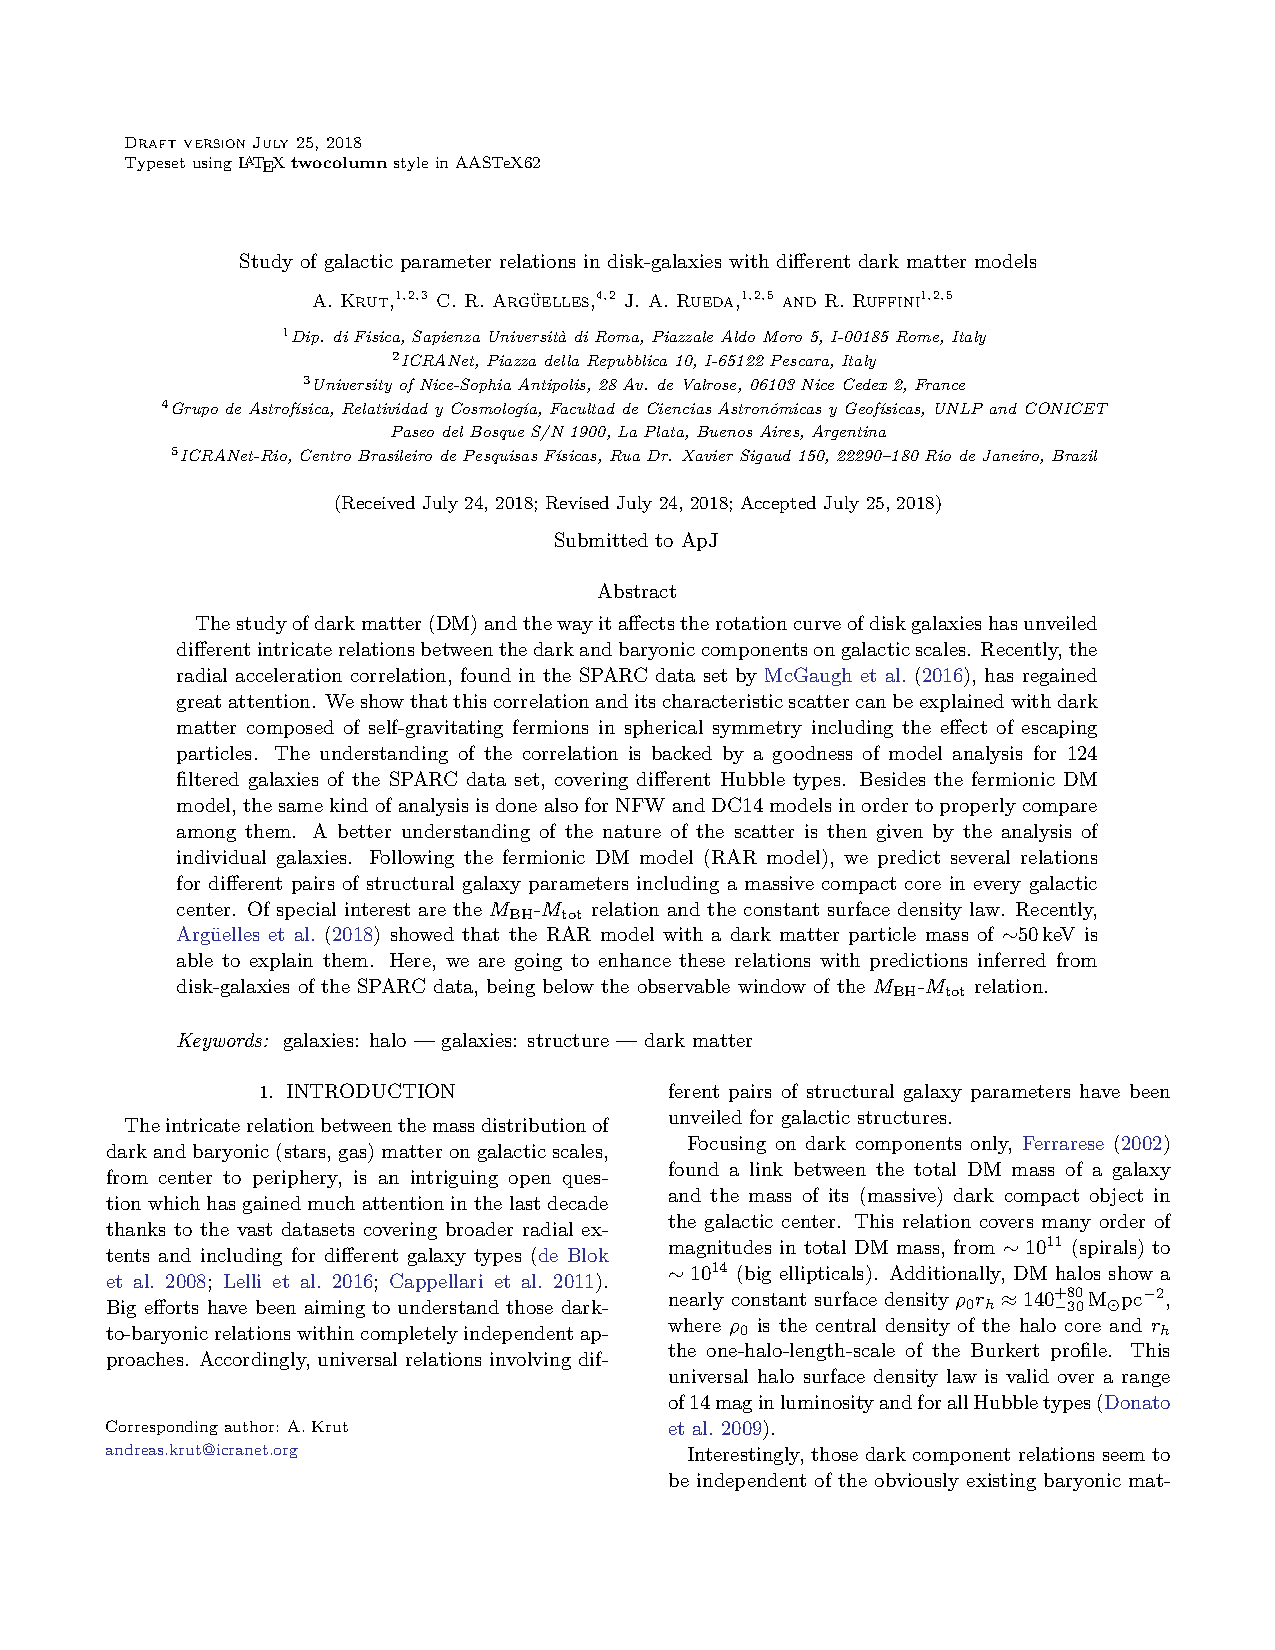
\includegraphics[width=\hsize]{\ROOTPATH/main.pdf}%
	\caption{Goodness of model analysis for galaxies showing one clear maximum in the outer halo RC, where DM typically dominates. This condition is fulfilled by 44 galaxies (see e.g. UGC05986 in \cref{fig:benchmark:total-rotation-curves}). We count the population of fitted galaxies having a reduced $\chi^2$ smaller than a given one. The normalized population (step-like) follows nearly a log-normal distribution (solid) characterized by the mean value $\hat \chi^2_r$. The shaded regions span the $\SI{95}{\percent}$ confidence interval of the best-fitted $\hat \chi^2_r$.}%
	\label{fig:goodness:with-cutoff}
\end{figure}